% In this chapter discuss functional requirements
% This is worth a lot so let's nail it
\chapter{Functional Requirements Specification}


% Who has a stake in the project?
% IE prospective users, possibly the finance
% backend people, possibly companies...
\section{Stakeholders}

The target demographic for the software described tends to be centered on students and
first time investors. That being said, it is likely to see the software expand to take
a large role in both university and pre-university classrooms, as a means of teaching
general financial concepts. It would not be unlikely to see the game further expand to
a larger range of users than other similar software due to increased functionality,
addition of achievement and leaderboards, and ability to join with or without league
functionality. Specifically, the addition of achievements leaves the user with the
desire to return and spend additional time trading on the software.\\

The league will be a free service with the intention of eventually moving to a
subtle-advertisement platform which will have no impact on the user. Once a
substantial enough user-base is generated, it will not be unlikely to see
advertisements begin to commence in order to bring revenue to the company. As a free
service (with eventual advertisements) we expect the platform to attract the greatest
number of users, and due to increased functionality, keep said users on the platform
for the greatest amount of time. The software is targeted not only at students and
potential investors, but at nearly everyone who desires to gain a greater understanding
of the financial industry as well as those who would simply like to practice trading
before executing in the real market.\\
 % no typos here...

% Who are some actors and what are their goals?
% I'm filling this from Nick's use cases
% but there could be even more
% Probably include a new file 
\section{Actors and Goals}

\subsection{Guest}
A visitor to the website who has either not logged in or just a simple visitor
\begin{itemize}
\item[--] Register and create an account using OpenID/OAuth2
\item[--] View the latest trades
\end{itemize}

\subsection{Investor}
A user who has an account in our servers and is logged in to their account
\begin{itemize}
\item[--] Research the latest updates in the market
\item[--] View their portfolio
\item[--] Execute orders of any kind
\item[--] Join/create a league
\item[--] Take part in competitions
\end{itemize}

\subsection{League Administrator}
Manages the leagues that they have created
\begin{itemize}
\item[--] Can set league to be public/private
\item[--] Set the rules for the league
\end{itemize}

\subsection{Database System}
Holds the information for the accounts of all users
\begin{itemize}
\item[--] Insert information as accounts are created
\item[--] Push data back to views about users/events
\item[--] Store new data about about users/events
\end{itemize}

\subsection{Financial API}
Gives the stocks in our database up to date prices
\begin{itemize}
\item[--] Fetch real world information and update our database accordingly
\end{itemize}

\subsection{Site Administrator}
Manages the overall website
\begin{itemize}
\item[--] Ensure fair competition between leagues/players
\end{itemize}

\subsection{Browser}
The middleman between user and system
\begin{itemize}
\item[--] Present data to the user
\item[--] Retrieve data from the user
\end{itemize}

\subsection{Yahoo! Finance}
The unit that knows about current financial statistics
\begin{itemize}
\item[--] Retrieve data about stocks
\end{itemize}

\subsection{Queueing System}
A subsystem for scheduling orders so as not to block user
interactions.
\begin{itemize}
\item[--] Place orders to be executed or canceled asynchronously
\item[--] Schedule events and mailings for system
\end{itemize}


\iffalse
\begin{figure}
\centering
\includegraphics[width=5.5in]{./Diagrams/UseCaseDiagram.png}
\caption{This graphic illustrates the relationships between the core actors of our platform.}
\end{figure}

% This is for the use cases
% These take up a lot so should be in another file
\section{Use Cases}

\input{./tex/fulldress}

\section{System Sequence Diagrams}

NEED DIAGRAMS FOR THIS SECTION!!!!!



In the following sequence diagrams, we describe exactly the interactions between the key
actors our system. It is important to note that most of the interaction between the
user and system is facilitated by the browser. The user, through filling forms and button
clicks, instructs the browser which requests to make to the system.
In turn, the system communicates with the database to request the desired data,
takes any required actions, and delivers the data to the browser for presentation to the user. \\


UC-1 – Register/create an account
When the user navigates to the login/ register accounts page, this use case
is triggered. The system makes it necessary to have an account before using
Paramount Investments leagues. The System then takes the information that the
user has input and sends them to the database, which then sends it back to the
system to display on the screen to the user. If the system finds that the user that is
registering with the same credentials as an existing account, the system throws up
an error appropriately.\\

UC-2 – Create/ Join a league
This use case is triggered when the user navigates to the create league page.
The user requests the system to create a league, which then sends appropriate
data to the database. Once the data is stored successfully, the database sends a
confirmation back to the system, which then displays an appropriate message to the
user. If the user wants to join a league, the user requests the system appropriately,
which then sends the data to the database regarding the right league and if
successful sends the confirmation to the user.\\

UC-3 – View Market Data
When the user navigates to the research stock page, this use case is triggered. The
user specifies to the system exactly what market data they would like to view. If
the user wants to research off the company’s website, then user will click on the
hyperlink present in the system. If the user wants to view the data through the
interface that Paramount Investment Provides, the system then pulls information
from the Yahoo Finance API and then sends it back to the system to display to the
user.\\

UC-4 – Manage Portfolio
This use case is triggered when the user goes to his/her own portfolio page. The
user navigates to the view portfolio page. The system then requests the database
to retrieve the user’s information. Once the database sends this data back to the
system, the system displays it to the user. The user is now free to modify aspects of
his/her portfolio. Once the user is finished modifying/updating their portfolio, the
system will send the changes to the database, which will then store the information
and save it.\\

UC-5 – Place a market order
This use case is triggered when the user goes to place a market order in the place
order page. The user selects a league to place the order into. The system then
displays the information to the user, who then requests to place a market order.
The system then queries to Yahoo Finance API to retrieve information about the
stock prices. The system then takes that information and processes it with what
the user wants to do. If the order is completed successfully, it is appropriately
displayed.\\

UC-6 – Take administrative Actions
This use case is triggered when the administrator of the website/ league wants
to take action. The system first checks if the user logging in has administrative
privileges in their respective group. If so, the system then looks in the database
to check for any logged conflicts. If there are unresolved conflicts, the database
returns them and then user can then view the conflicts. If there are no conflicts to
be resolved, then display so appropriately to the administrator/logged in user.\\

UC-7 – Manage League Settings
This use case is triggered when the manager of a league wants to change the league
settings. The system first checks to see if the user that is logged in, is the league
manager and if so, the grants the user privilege to change league settings. The user
then requests to change the league settings. The system retrieves the league data
and modifies it as the user has requested.\\



\iffalse
\begin{figure}
\centering
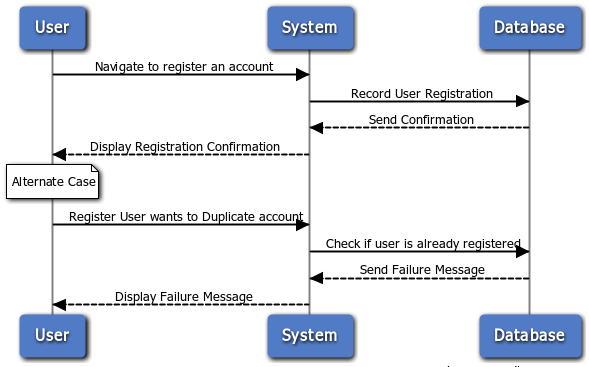
\includegraphics[width=5.5in]{./Diagrams/SystemSequenceDiagrams/uc1.png}
\caption{See UC-1 on page \pageref{UC-1}. When the user navigates to the league listing page, they invoke this use case. The user initiates a request to view all the public leagues and the system retrieves them from the database. Then, they are presented to the user who is given the option to join any valid league.}
\end{figure}

\begin{figure}
\centering
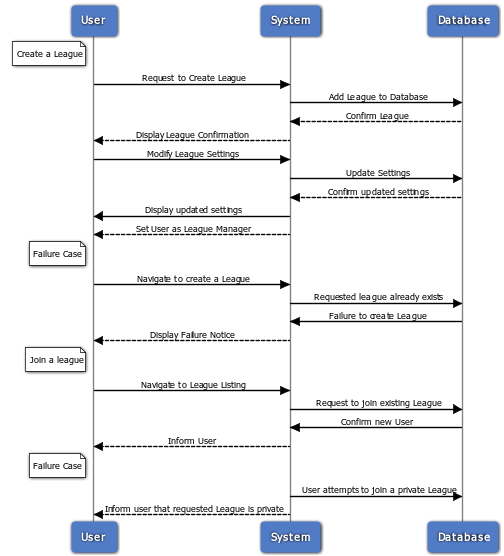
\includegraphics[width=5.5in]{./Diagrams/SystemSequenceDiagrams/uc2.png}
\caption{See UC-2 on page \pageref{UC-2}. This is sequence of events that occur when a league manager alters the league settings. The system fetches the current settings from the database and returns them to the browser. It also ensures that the user attempting this change is a league manager. Then, the user can initiate a request to change the settings which will be enacted out by the system. If the league manager changes the status of a user within the league, the system notifies that user.}
\end{figure}

\begin{figure}
\centering
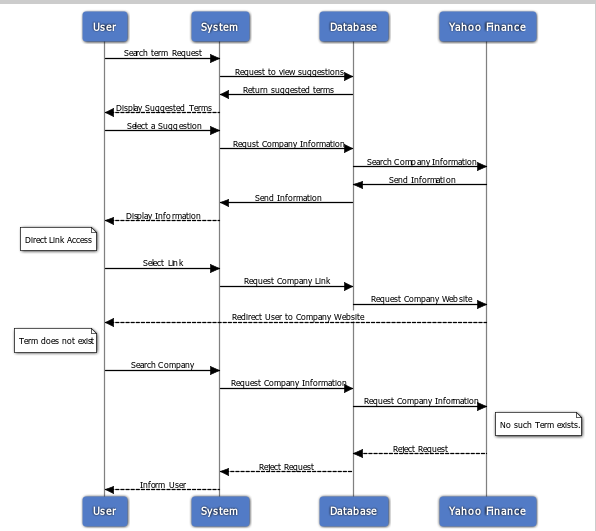
\includegraphics[width=5.5in]{./Diagrams/SystemSequenceDiagrams/uc3.png}
\caption{See UC-3 on page \pageref{UC-3}. When the user desires to research companies, this is the sequence that follows. The user is able to search and browse for companies. They can also get to a company's page through a direct link. Yahoo! Finance responds to requests and delivers data to our system which is then transferred to the browser and fills out a company profile.}
\end{figure}

\begin{figure}
\centering
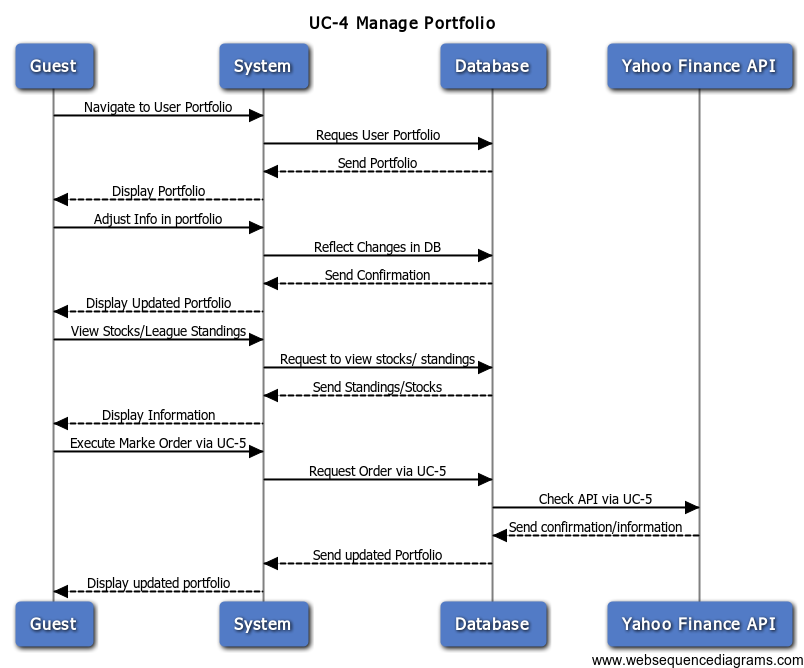
\includegraphics[width=5.5in]{./Diagrams/SystemSequenceDiagrams/uc4.png}
\caption{See for UC-4 on page \pageref{UC-4}. This sequence encompasses the bread and butter of our application--market orders. The user selects a league in which to place an order, fills out a prompt in the browser which then submits the request to the system. The system inserts the order into the database and enqueues it (the queuing system will be elaborated upon in a later section). Once the order resolves or expires, the database notifies the system and the user's portfolio is updated accordingly.}
\end{figure}

\begin{figure}
\centering
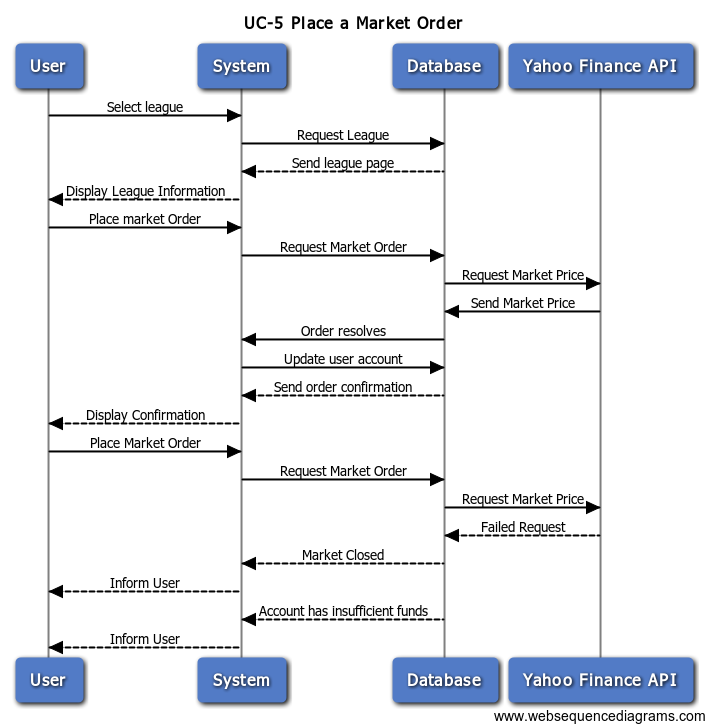
\includegraphics[width=5.5in]{./Diagrams/SystemSequenceDiagrams/uc5.png}
\caption{See UC-5 on page \pageref{UC-5}. This use case is relatively straightforward. The user browses to a league member's portfolio, and the browser submits a request to the database for that portfolio's inormation.}
\end{figure}

\begin{figure}
\centering
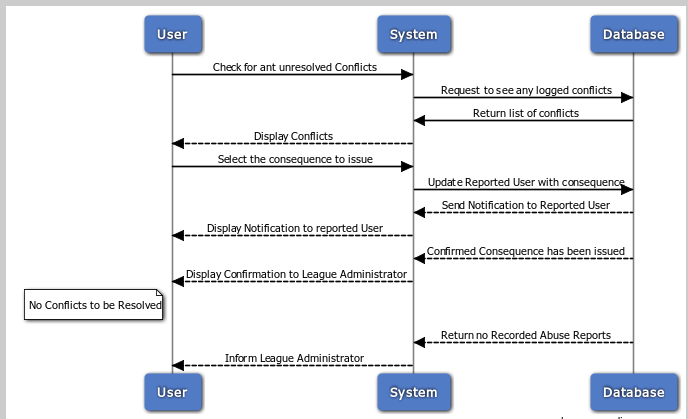
\includegraphics[width=5.5in]{./Diagrams/SystemSequenceDiagrams/uc6.png}
\caption{See UC-6 on page \pageref{UC-6}. Another simple use case. The user simply navigates to the tutorial page, which is populated by the system.}
\end{figure}

\begin{figure}
\centering
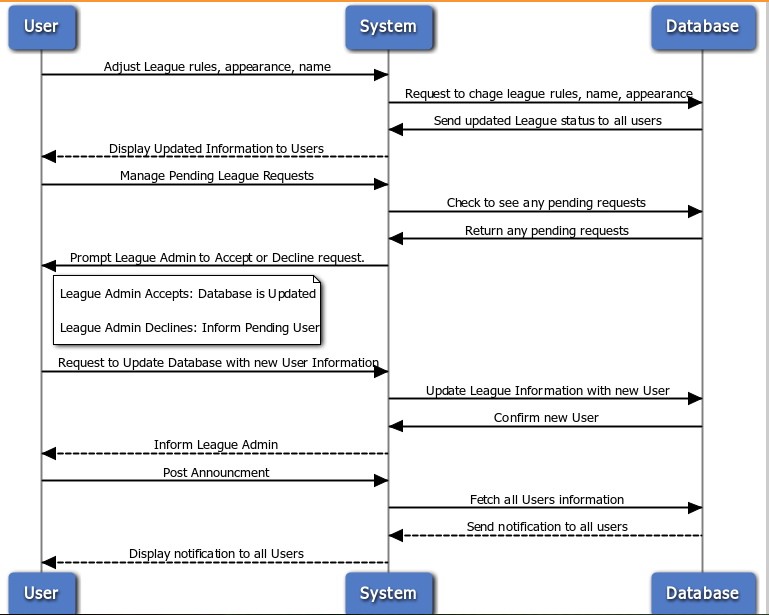
\includegraphics[width=5.5in]{./Diagrams/SystemSequenceDiagrams/uc7.png}
\caption{See UC-7 on page \pageref{UC-7}. When a site administrator navigates to observe any outstanding abuse reports, this flow of events is initiated. The database delivers all outstanding reports to the system which then populates them in the browser. If the administrator decides to take an action, the status change is reflected in the database, and the system notifies the user of whatever action was taken against them.}
\end{figure}
\fi

\fi
